\section{自己紹介}
\begin{itemize}
	\item 職業:オフィス家具メーカーに2001年入社、2003年~CAEを担当
	\item オープンCAE歴
	      \begin{itemize}
		      \item 2011年05月:第32回関西CAE懇話会「CAEの新しい波、オープンソースとFOCUSスパコン」でオープンCAEを知る
		            \begin{itemize}
			            \item 実習講座「オープンCAEから始める構造解析CAEの基本」に参加し、岐阜高専の柴田先生、DEXCS、Adventureを知る
		            \end{itemize}
		      \item 2011年08月:関西地区の解析塾「はじめてのオープンCAE」を受講し、Salome-Mecaを知る
		      \item 2011年11月:CAE懇話会の「Salome-Meca活用研究会」が発足、参加
		      \item 2012年08月:第16回「オープンCAE勉強会@岐阜(夏合宿2)」に初参加
		      \item 2012年XX月:「オープンCAE学会」に入会
		      \item 2013年02月:第20回「オープンCAE勉強会@関西」に初参加
		      \item 2016年10月:第09回「オープンCAE勉強会@関東(構造など)」に初参加
	      \end{itemize}
	\item 情報発信
	      \begin{itemize}
		      \item Twitter \href{https://twitter.com/Jun_Tatsuno}{@Jun\_Tatsuno}
		      \item Qiita \href{https://qiita.com/Jun_Tatsuno}{@Jun\_Tatsuno}
		      \item GitHub \href{https://github.com/JunTatsuno/}{@JunTatsuno}
		      \item Speaker Deck \href{https://speakerdeck.com/juntatsuno/}{@JunTatsuno}
		      \item \href{https://www.youtube.com/playlist?list=PL3Ey4GcIvUy-2_ZMZ7dG_Wez4H__rin5c}{YouTube}
	      \end{itemize}
\end{itemize}
\section{Salome-Mecaとは}
\begin{itemize}
	\item EDF(フランス電力公社)が提供している、Linuxベースのオープンソース構造・熱解析ソフト
	      \begin{itemize}
		      \item Code\_Aster:解析ソルバー
		      \item Salome-Meca:プリポストを中心とした統合プラットフォーム(SALOME Platform)に、Code\_Asterをモジュールとして組み込んだもの
	      \end{itemize}
	      \begin{figure}[htbp]
		      % 	\caption{}
		      % 	\label{}
		      \centering
		      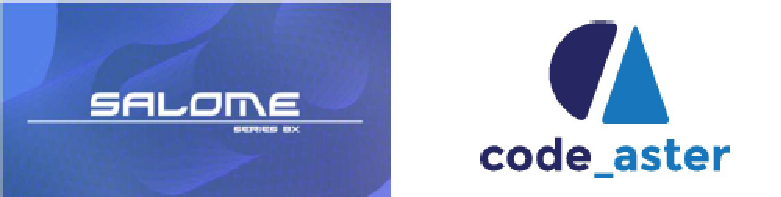
\includegraphics[width=0.4\linewidth]{fig/salome-aster.pdf}
	      \end{figure}
	\item Code\_Asterは、構造力学、熱力学を中心に非常に高度で多彩な機能と400を超える要素(1次元、2次元、3次元ほか)を有しています。また、2,000以上のテストケースと、13,000ページ以上のドキュメント(使用方法、テクニック、理論的背景)、公式フォーラムなどがあり、他のオープンソースCAEソフトと較べてサポート体制が充実しているのが特長です。
	\item Code\_Aster \& Salome-Meca日本語解説より
	      \href{https://sites.google.com/site/codeastersalomemeca/home}{https://sites.google.com/site/codeastersalomemeca/home}
\end{itemize}